\documentclass[1p]{elsarticle_modified}
%\bibliographystyle{elsarticle-num}

%\usepackage[colorlinks]{hyperref}
%\usepackage{abbrmath_seonhwa} %\Abb, \Ascr, \Acal ,\Abf, \Afrak
\usepackage{amsfonts}
\usepackage{amssymb}
\usepackage{amsmath}
\usepackage{amsthm}
\usepackage{scalefnt}
\usepackage{amsbsy}
\usepackage{kotex}
\usepackage{caption}
\usepackage{subfig}
\usepackage{color}
\usepackage{graphicx}
\usepackage{xcolor} %% white, black, red, green, blue, cyan, magenta, yellow
\usepackage{float}
\usepackage{setspace}
\usepackage{hyperref}

\usepackage{tikz}
\usetikzlibrary{arrows}

\usepackage{multirow}
\usepackage{array} % fixed length table
\usepackage{hhline}

%%%%%%%%%%%%%%%%%%%%%
\makeatletter
\renewcommand*\env@matrix[1][\arraystretch]{%
	\edef\arraystretch{#1}%
	\hskip -\arraycolsep
	\let\@ifnextchar\new@ifnextchar
	\array{*\c@MaxMatrixCols c}}
\makeatother %https://tex.stackexchange.com/questions/14071/how-can-i-increase-the-line-spacing-in-a-matrix
%%%%%%%%%%%%%%%

\usepackage[normalem]{ulem}

\newcommand{\msout}[1]{\ifmmode\text{\sout{\ensuremath{#1}}}\else\sout{#1}\fi}
%SOURCE: \msout is \stkout macro in https://tex.stackexchange.com/questions/20609/strikeout-in-math-mode

\newcommand{\cancel}[1]{
	\ifmmode
	{\color{red}\msout{#1}}
	\else
	{\color{red}\sout{#1}}
	\fi
}

\newcommand{\add}[1]{
	{\color{blue}\uwave{#1}}
}

\newcommand{\replace}[2]{
	\ifmmode
	{\color{red}\msout{#1}}{\color{blue}\uwave{#2}}
	\else
	{\color{red}\sout{#1}}{\color{blue}\uwave{#2}}
	\fi
}

\newcommand{\Sol}{\mathcal{S}} %segment
\newcommand{\D}{D} %diagram
\newcommand{\A}{\mathcal{A}} %arc


%%%%%%%%%%%%%%%%%%%%%%%%%%%%%5 test

\def\sl{\operatorname{\textup{SL}}(2,\Cbb)}
\def\psl{\operatorname{\textup{PSL}}(2,\Cbb)}
\def\quan{\mkern 1mu \triangleright \mkern 1mu}

\theoremstyle{definition}
\newtheorem{thm}{Theorem}[section]
\newtheorem{prop}[thm]{Proposition}
\newtheorem{lem}[thm]{Lemma}
\newtheorem{ques}[thm]{Question}
\newtheorem{cor}[thm]{Corollary}
\newtheorem{defn}[thm]{Definition}
\newtheorem{exam}[thm]{Example}
\newtheorem{rmk}[thm]{Remark}
\newtheorem{alg}[thm]{Algorithm}

\newcommand{\I}{\sqrt{-1}}
\begin{document}

%\begin{frontmatter}
%
%\title{Boundary parabolic representations of knots up to 8 crossings}
%
%%% Group authors per affiliation:
%\author{Yunhi Cho} 
%\address{Department of Mathematics, University of Seoul, Seoul, Korea}
%\ead{yhcho@uos.ac.kr}
%
%
%\author{Seonhwa Kim} %\fnref{s_kim}}
%\address{Center for Geometry and Physics, Institute for Basic Science, Pohang, 37673, Korea}
%\ead{ryeona17@ibs.re.kr}
%
%\author{Hyuk Kim}
%\address{Department of Mathematical Sciences, Seoul National University, Seoul 08826, Korea}
%\ead{hyukkim@snu.ac.kr}
%
%\author{Seokbeom Yoon}
%\address{Department of Mathematical Sciences, Seoul National University, Seoul, 08826,  Korea}
%\ead{sbyoon15@snu.ac.kr}
%
%\begin{abstract}
%We find all boundary parabolic representation of knots up to 8 crossings.
%
%\end{abstract}
%\begin{keyword}
%    \MSC[2010] 57M25 
%\end{keyword}
%
%\end{frontmatter}

%\linenumbers
%\tableofcontents
%
\newcommand\colored[1]{\textcolor{white}{\rule[-0.35ex]{0.8em}{1.4ex}}\kern-0.8em\color{red} #1}%
%\newcommand\colored[1]{\textcolor{white}{ #1}\kern-2.17ex	\textcolor{white}{ #1}\kern-1.81ex	\textcolor{white}{ #1}\kern-2.15ex\color{red}#1	}

{\Large $\underline{12a_{0650}~(K12a_{0650})}$}

\setlength{\tabcolsep}{10pt}
\renewcommand{\arraystretch}{1.6}
\vspace{1cm}\begin{tabular}{m{100pt}>{\centering\arraybackslash}m{274pt}}
\multirow{5}{120pt}{
	\centering
	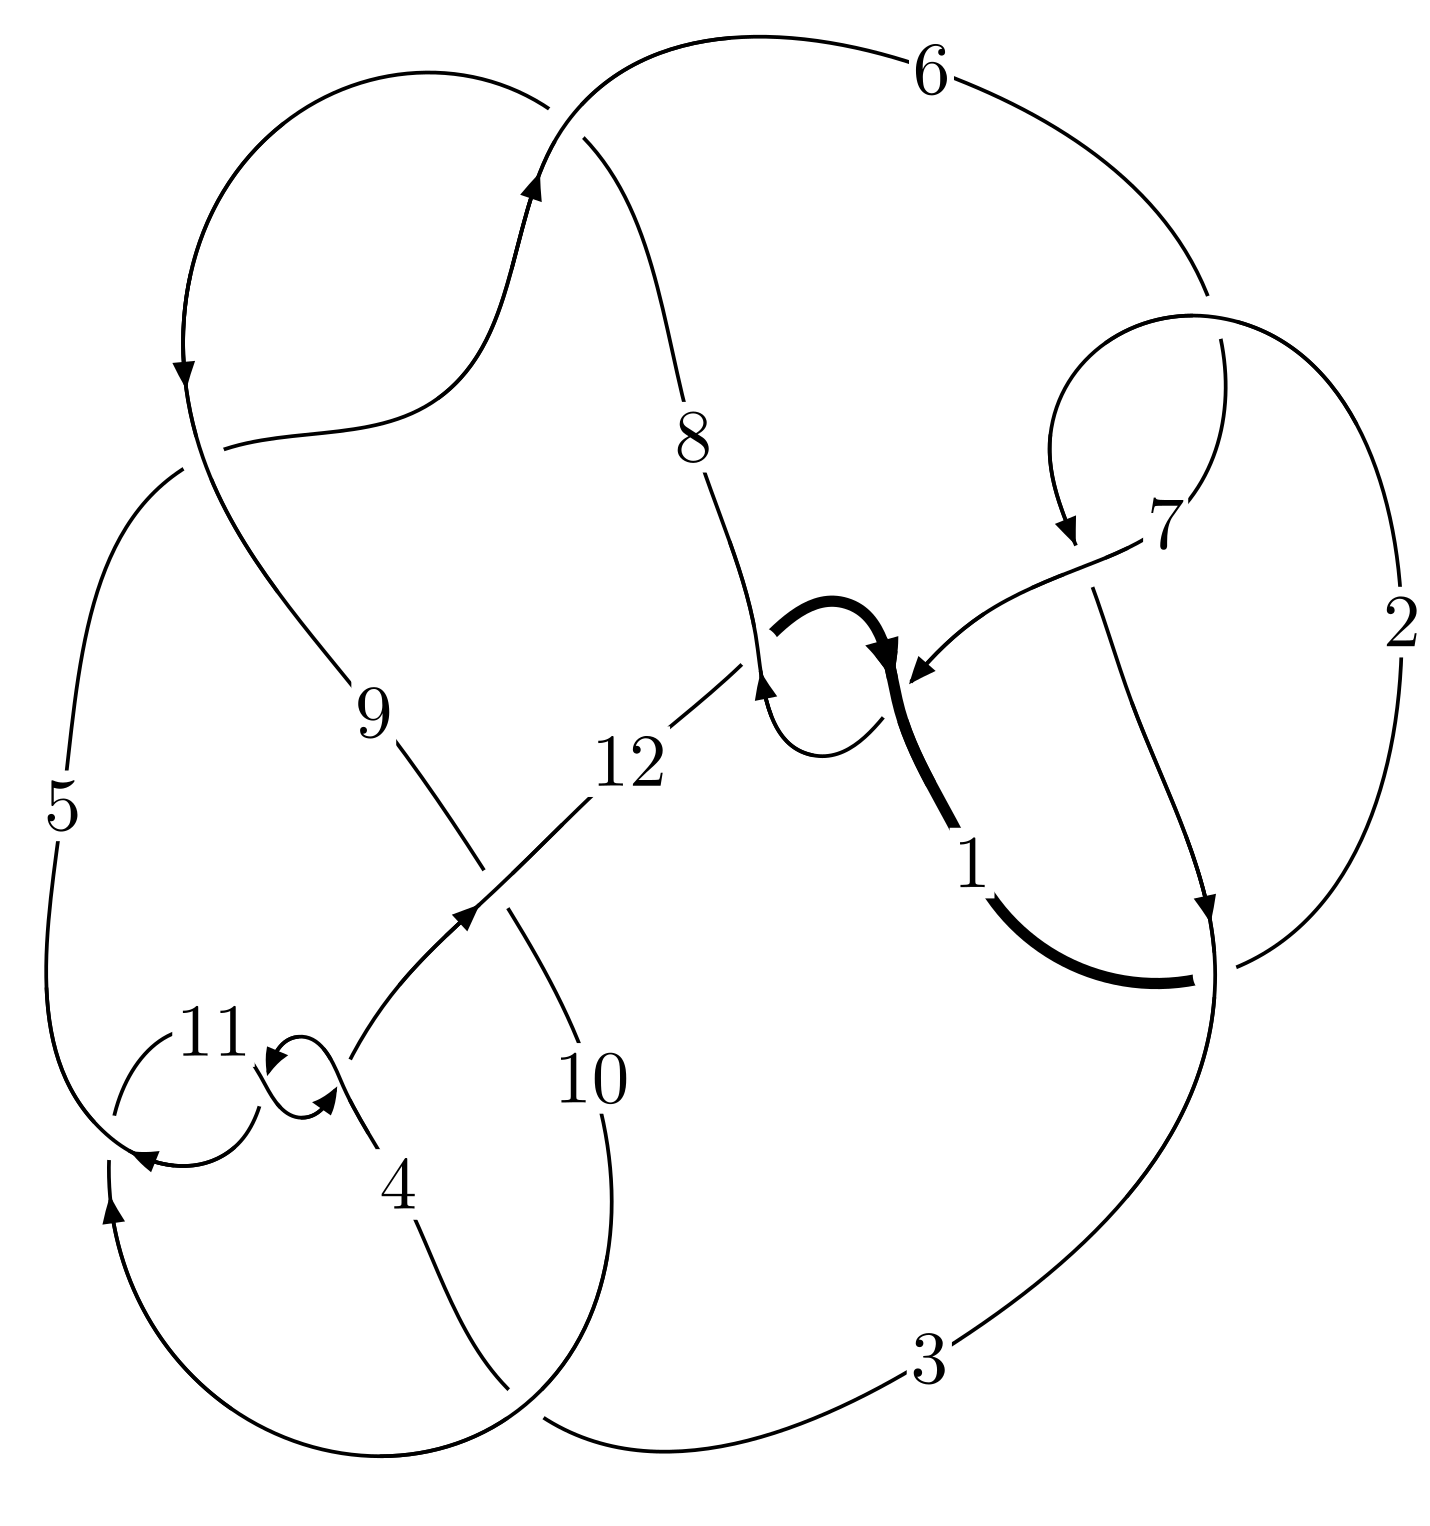
\includegraphics[width=112pt]{../../../GIT/diagram.site/Diagrams/png/1451_12a_0650.png}\\
\ \ \ A knot diagram\footnotemark}&
\allowdisplaybreaks
\textbf{Linearized knot diagam} \\
\cline{2-2}
 &
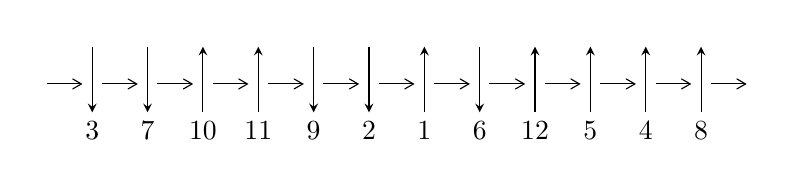
\begin{tikzpicture}[x=20pt, y=17pt]
	% nodes
	\node (C0) at (0, 0) {};
	\node (C1) at (1, 0) {};
	\node (C1U) at (1, +1) {};
	\node (C1D) at (1, -1) {3};

	\node (C2) at (2, 0) {};
	\node (C2U) at (2, +1) {};
	\node (C2D) at (2, -1) {7};

	\node (C3) at (3, 0) {};
	\node (C3U) at (3, +1) {};
	\node (C3D) at (3, -1) {10};

	\node (C4) at (4, 0) {};
	\node (C4U) at (4, +1) {};
	\node (C4D) at (4, -1) {11};

	\node (C5) at (5, 0) {};
	\node (C5U) at (5, +1) {};
	\node (C5D) at (5, -1) {9};

	\node (C6) at (6, 0) {};
	\node (C6U) at (6, +1) {};
	\node (C6D) at (6, -1) {2};

	\node (C7) at (7, 0) {};
	\node (C7U) at (7, +1) {};
	\node (C7D) at (7, -1) {1};

	\node (C8) at (8, 0) {};
	\node (C8U) at (8, +1) {};
	\node (C8D) at (8, -1) {6};

	\node (C9) at (9, 0) {};
	\node (C9U) at (9, +1) {};
	\node (C9D) at (9, -1) {12};

	\node (C10) at (10, 0) {};
	\node (C10U) at (10, +1) {};
	\node (C10D) at (10, -1) {5};

	\node (C11) at (11, 0) {};
	\node (C11U) at (11, +1) {};
	\node (C11D) at (11, -1) {4};

	\node (C12) at (12, 0) {};
	\node (C12U) at (12, +1) {};
	\node (C12D) at (12, -1) {8};
	\node (C13) at (13, 0) {};

	% arrows
	\draw[->,>={angle 60}]
	(C0) edge (C1) (C1) edge (C2) (C2) edge (C3) (C3) edge (C4) (C4) edge (C5) (C5) edge (C6) (C6) edge (C7) (C7) edge (C8) (C8) edge (C9) (C9) edge (C10) (C10) edge (C11) (C11) edge (C12) (C12) edge (C13) ;	\draw[->,>=stealth]
	(C1U) edge (C1D) (C2U) edge (C2D) (C3D) edge (C3U) (C4D) edge (C4U) (C5U) edge (C5D) (C6U) edge (C6D) (C7D) edge (C7U) (C8U) edge (C8D) (C9D) edge (C9U) (C10D) edge (C10U) (C11D) edge (C11U) (C12D) edge (C12U) ;
	\end{tikzpicture} \\
\hhline{~~} \\& 
\textbf{Solving Sequence} \\ \cline{2-2} 
 &
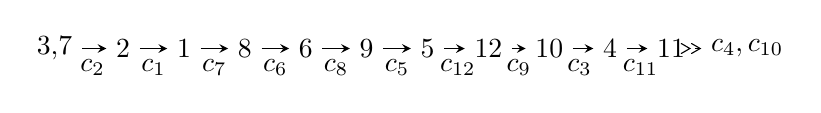
\begin{tikzpicture}[x=22pt, y=7pt]
	% node
	\node (A0) at (-1/8, 0) {3,7};
	\node (A1) at (1, 0) {2};
	\node (A2) at (2, 0) {1};
	\node (A3) at (3, 0) {8};
	\node (A4) at (4, 0) {6};
	\node (A5) at (5, 0) {9};
	\node (A6) at (6, 0) {5};
	\node (A7) at (7, 0) {12};
	\node (A8) at (8, 0) {10};
	\node (A9) at (9, 0) {4};
	\node (A10) at (10, 0) {11};
	\node (C1) at (1/2, -1) {$c_{2}$};
	\node (C2) at (3/2, -1) {$c_{1}$};
	\node (C3) at (5/2, -1) {$c_{7}$};
	\node (C4) at (7/2, -1) {$c_{6}$};
	\node (C5) at (9/2, -1) {$c_{8}$};
	\node (C6) at (11/2, -1) {$c_{5}$};
	\node (C7) at (13/2, -1) {$c_{12}$};
	\node (C8) at (15/2, -1) {$c_{9}$};
	\node (C9) at (17/2, -1) {$c_{3}$};
	\node (C10) at (19/2, -1) {$c_{11}$};
	\node (A11) at (45/4, 0) {$c_{4},c_{10}$};

	% edge
	\draw[->,>=stealth]	
	(A0) edge (A1) (A1) edge (A2) (A2) edge (A3) (A3) edge (A4) (A4) edge (A5) (A5) edge (A6) (A6) edge (A7) (A7) edge (A8) (A8) edge (A9) (A9) edge (A10) ;
	\draw[->>,>={angle 60}]	
	(A10) edge (A11);
\end{tikzpicture} \\ 

\end{tabular} \\

\footnotetext{
The image of knot diagram is generated by the software ``\textbf{Draw programme}" developed by Andrew Bartholomew(\url{http://www.layer8.co.uk/maths/draw/index.htm\#Running-draw}), where we modified some parts for our purpose(\url{https://github.com/CATsTAILs/LinksPainter}).
}\phantom \\ \newline 
\centering \textbf{Ideals for irreducible components\footnotemark of $X_{\text{par}}$} 
 
\begin{align*}
I^u_{1}&=\langle 
u^{82}- u^{81}+\cdots- u+1\rangle \\
\\
\end{align*}
\raggedright * 1 irreducible components of $\dim_{\mathbb{C}}=0$, with total 82 representations.\\
\footnotetext{All coefficients of polynomials are rational numbers. But the coefficients are sometimes approximated in decimal forms when there is not enough margin.}
\newpage
\renewcommand{\arraystretch}{1}
\centering \section*{I. $I^u_{1}= \langle u^{82}- u^{81}+\cdots- u+1 \rangle$}
\flushleft \textbf{(i) Arc colorings}\\
\begin{tabular}{m{7pt} m{180pt} m{7pt} m{180pt} }
\flushright $a_{3}=$&$\begin{pmatrix}1\\0\end{pmatrix}$ \\
\flushright $a_{7}=$&$\begin{pmatrix}0\\u\end{pmatrix}$ \\
\flushright $a_{2}=$&$\begin{pmatrix}1\\- u^2\end{pmatrix}$ \\
\flushright $a_{1}=$&$\begin{pmatrix}- u^2+1\\- u^2\end{pmatrix}$ \\
\flushright $a_{8}=$&$\begin{pmatrix}u^5-2 u^3+u\\u^5- u^3+u\end{pmatrix}$ \\
\flushright $a_{6}=$&$\begin{pmatrix}u\\- u^3+u\end{pmatrix}$ \\
\flushright $a_{9}=$&$\begin{pmatrix}- u^9+2 u^7- u^5-2 u^3+u\\u^{11}-3 u^9+4 u^7- u^5- u^3+u\end{pmatrix}$ \\
\flushright $a_{5}=$&$\begin{pmatrix}u^{17}-4 u^{15}+7 u^{13}-4 u^{11}-3 u^9+6 u^7-2 u^5+u\\- u^{19}+5 u^{17}-12 u^{15}+15 u^{13}-9 u^{11}- u^9+4 u^7-2 u^5- u^3+u\end{pmatrix}$ \\
\flushright $a_{12}=$&$\begin{pmatrix}- u^8+3 u^6-3 u^4+1\\- u^8+2 u^6-2 u^4\end{pmatrix}$ \\
\flushright $a_{10}=$&$\begin{pmatrix}u^{27}-8 u^{25}+\cdots-3 u^3+2 u\\u^{27}-7 u^{25}+\cdots- u^3+u\end{pmatrix}$ \\
\flushright $a_{4}=$&$\begin{pmatrix}- u^{54}+15 u^{52}+\cdots-2 u^2+1\\- u^{54}+14 u^{52}+\cdots+2 u^4- u^2\end{pmatrix}$ \\
\flushright $a_{11}=$&$\begin{pmatrix}u^{63}-16 u^{61}+\cdots-4 u^3+2 u\\- u^{65}+17 u^{63}+\cdots-2 u^3+u\end{pmatrix}$\\&\end{tabular}
\flushleft \textbf{(ii) Obstruction class $= -1$}\\~\\
\flushleft \textbf{(iii) Cusp Shapes $= 4 u^{80}-84 u^{78}+\cdots+8 u+2$}\\~\\
\newpage\renewcommand{\arraystretch}{1}
\flushleft \textbf{(iv) u-Polynomials at the component}\newline \\
\begin{tabular}{m{50pt}|m{274pt}}
Crossings & \hspace{64pt}u-Polynomials at each crossing \\
\hline $$\begin{aligned}c_{1}\end{aligned}$$&$\begin{aligned}
&u^{82}+43 u^{81}+\cdots+3 u+1
\end{aligned}$\\
\hline $$\begin{aligned}c_{2},c_{6}\end{aligned}$$&$\begin{aligned}
&u^{82}- u^{81}+\cdots- u+1
\end{aligned}$\\
\hline $$\begin{aligned}c_{3}\end{aligned}$$&$\begin{aligned}
&u^{82}+u^{81}+\cdots-5 u+2
\end{aligned}$\\
\hline $$\begin{aligned}c_{4},c_{10},c_{11}\end{aligned}$$&$\begin{aligned}
&u^{82}- u^{81}+\cdots- u+1
\end{aligned}$\\
\hline $$\begin{aligned}c_{5},c_{8}\end{aligned}$$&$\begin{aligned}
&u^{82}-7 u^{81}+\cdots-383 u+37
\end{aligned}$\\
\hline $$\begin{aligned}c_{7},c_{12}\end{aligned}$$&$\begin{aligned}
&u^{82}-3 u^{81}+\cdots-55 u+56
\end{aligned}$\\
\hline $$\begin{aligned}c_{9}\end{aligned}$$&$\begin{aligned}
&u^{82}+19 u^{81}+\cdots+5211 u+283
\end{aligned}$\\
\hline
\end{tabular}\\~\\
\newpage\renewcommand{\arraystretch}{1}
\flushleft \textbf{(v) Riley Polynomials at the component}\newline \\
\begin{tabular}{m{50pt}|m{274pt}}
Crossings & \hspace{64pt}Riley Polynomials at each crossing \\
\hline $$\begin{aligned}c_{1}\end{aligned}$$&$\begin{aligned}
&y^{82}-7 y^{81}+\cdots+9 y+1
\end{aligned}$\\
\hline $$\begin{aligned}c_{2},c_{6}\end{aligned}$$&$\begin{aligned}
&y^{82}-43 y^{81}+\cdots-3 y+1
\end{aligned}$\\
\hline $$\begin{aligned}c_{3}\end{aligned}$$&$\begin{aligned}
&y^{82}-3 y^{81}+\cdots-25 y+4
\end{aligned}$\\
\hline $$\begin{aligned}c_{4},c_{10},c_{11}\end{aligned}$$&$\begin{aligned}
&y^{82}+73 y^{81}+\cdots-3 y+1
\end{aligned}$\\
\hline $$\begin{aligned}c_{5},c_{8}\end{aligned}$$&$\begin{aligned}
&y^{82}+53 y^{81}+\cdots+11449 y+1369
\end{aligned}$\\
\hline $$\begin{aligned}c_{7},c_{12}\end{aligned}$$&$\begin{aligned}
&y^{82}+57 y^{81}+\cdots+137423 y+3136
\end{aligned}$\\
\hline $$\begin{aligned}c_{9}\end{aligned}$$&$\begin{aligned}
&y^{82}+13 y^{81}+\cdots+2040325 y+80089
\end{aligned}$\\
\hline
\end{tabular}\\~\\
\newpage\flushleft \textbf{(vi) Complex Volumes and Cusp Shapes}
$$\begin{array}{c|c|c}  
\text{Solutions to }I^u_{1}& \I (\text{vol} + \sqrt{-1}CS) & \text{Cusp shape}\\
 \hline 
\begin{aligned}
u &= \phantom{-}0.955352 + 0.293882 I\end{aligned}
 & -0.49000 - 3.37255 I & \phantom{-0.000000 -}0. + 7.86263 I \\ \hline\begin{aligned}
u &= \phantom{-}0.955352 - 0.293882 I\end{aligned}
 & -0.49000 + 3.37255 I & \phantom{-0.000000 } 0. - 7.86263 I \\ \hline\begin{aligned}
u &= \phantom{-}0.816926 + 0.582560 I\end{aligned}
 & -0.09685 - 9.75450 I & \phantom{-0.000000 -}0. + 8.56550 I \\ \hline\begin{aligned}
u &= \phantom{-}0.816926 - 0.582560 I\end{aligned}
 & -0.09685 + 9.75450 I & \phantom{-0.000000 } 0. - 8.56550 I \\ \hline\begin{aligned}
u &= -0.804317 + 0.580383 I\end{aligned}
 & \phantom{-}5.07118 + 6.08583 I & \phantom{-}7.27321 - 7.72699 I \\ \hline\begin{aligned}
u &= -0.804317 - 0.580383 I\end{aligned}
 & \phantom{-}5.07118 - 6.08583 I & \phantom{-}7.27321 + 7.72699 I \\ \hline\begin{aligned}
u &= \phantom{-}0.976357 + 0.106548 I\end{aligned}
 & -6.89382 + 1.35042 I & -8.09485 + 0. I\phantom{ +0.000000I} \\ \hline\begin{aligned}
u &= \phantom{-}0.976357 - 0.106548 I\end{aligned}
 & -6.89382 - 1.35042 I & -8.09485 + 0. I\phantom{ +0.000000I} \\ \hline\begin{aligned}
u &= \phantom{-}0.780556 + 0.572028 I\end{aligned}
 & \phantom{-}3.12382 - 2.34167 I & \phantom{-}4.61313 + 2.84945 I \\ \hline\begin{aligned}
u &= \phantom{-}0.780556 - 0.572028 I\end{aligned}
 & \phantom{-}3.12382 + 2.34167 I & \phantom{-}4.61313 - 2.84945 I \\ \hline\begin{aligned}
u &= -0.813516 + 0.498678 I\end{aligned}
 & -3.07012 + 1.93466 I & \phantom{-0.000000 } 0. - 4.43003 I \\ \hline\begin{aligned}
u &= -0.813516 - 0.498678 I\end{aligned}
 & -3.07012 - 1.93466 I & \phantom{-0.000000 -}0. + 4.43003 I \\ \hline\begin{aligned}
u &= \phantom{-}0.760520 + 0.575296 I\end{aligned}
 & \phantom{-}3.18119 - 2.21323 I & \phantom{-}4.97236 + 4.23790 I \\ \hline\begin{aligned}
u &= \phantom{-}0.760520 - 0.575296 I\end{aligned}
 & \phantom{-}3.18119 + 2.21323 I & \phantom{-}4.97236 - 4.23790 I \\ \hline\begin{aligned}
u &= -0.733948 + 0.585447 I\end{aligned}
 & \phantom{-}5.27270 - 1.47770 I & \phantom{-}8.11976 + 0.84952 I \\ \hline\begin{aligned}
u &= -0.733948 - 0.585447 I\end{aligned}
 & \phantom{-}5.27270 + 1.47770 I & \phantom{-}8.11976 - 0.84952 I \\ \hline\begin{aligned}
u &= -1.038490 + 0.247739 I\end{aligned}
 & -5.58353 + 6.55182 I & \phantom{-0.000000 } 0 \\ \hline\begin{aligned}
u &= -1.038490 - 0.247739 I\end{aligned}
 & -5.58353 - 6.55182 I & \phantom{-0.000000 } 0 \\ \hline\begin{aligned}
u &= \phantom{-}0.718789 + 0.591071 I\end{aligned}
 & \phantom{-}0.18371 + 5.12454 I & \phantom{-}3.29871 - 1.93532 I \\ \hline\begin{aligned}
u &= \phantom{-}0.718789 - 0.591071 I\end{aligned}
 & \phantom{-}0.18371 - 5.12454 I & \phantom{-}3.29871 + 1.93532 I \\ \hline\begin{aligned}
u &= -0.870197 + 0.149170 I\end{aligned}
 & -1.47910 + 0.55712 I & -4.57771 - 0.31676 I \\ \hline\begin{aligned}
u &= -0.870197 - 0.149170 I\end{aligned}
 & -1.47910 - 0.55712 I & -4.57771 + 0.31676 I \\ \hline\begin{aligned}
u &= -1.062130 + 0.425517 I\end{aligned}
 & -5.33957 + 6.56153 I & \phantom{-0.000000 } 0 \\ \hline\begin{aligned}
u &= -1.062130 - 0.425517 I\end{aligned}
 & -5.33957 - 6.56153 I & \phantom{-0.000000 } 0 \\ \hline\begin{aligned}
u &= \phantom{-}1.093670 + 0.357724 I\end{aligned}
 & -0.62091 - 3.37016 I & \phantom{-0.000000 } 0 \\ \hline\begin{aligned}
u &= \phantom{-}1.093670 - 0.357724 I\end{aligned}
 & -0.62091 + 3.37016 I & \phantom{-0.000000 } 0 \\ \hline\begin{aligned}
u &= \phantom{-}0.186761 + 0.793781 I\end{aligned}
 & -3.11263 + 10.80720 I & \phantom{-}0.45907 - 6.86198 I \\ \hline\begin{aligned}
u &= \phantom{-}0.186761 - 0.793781 I\end{aligned}
 & -3.11263 - 10.80720 I & \phantom{-}0.45907 + 6.86198 I \\ \hline\begin{aligned}
u &= -0.190528 + 0.784354 I\end{aligned}
 & \phantom{-}2.19850 - 7.14289 I & \phantom{-}5.14145 + 6.39279 I \\ \hline\begin{aligned}
u &= -0.190528 - 0.784354 I\end{aligned}
 & \phantom{-}2.19850 + 7.14289 I & \phantom{-}5.14145 - 6.39279 I\\
 \hline 
 \end{array}$$\newpage$$\begin{array}{c|c|c}  
\text{Solutions to }I^u_{1}& \I (\text{vol} + \sqrt{-1}CS) & \text{Cusp shape}\\
 \hline 
\begin{aligned}
u &= -1.147130 + 0.343021 I\end{aligned}
 & -3.17720 + 0.08534 I & \phantom{-0.000000 } 0 \\ \hline\begin{aligned}
u &= -1.147130 - 0.343021 I\end{aligned}
 & -3.17720 - 0.08534 I & \phantom{-0.000000 } 0 \\ \hline\begin{aligned}
u &= \phantom{-}0.189777 + 0.763023 I\end{aligned}
 & \phantom{-}0.52237 + 3.32831 I & \phantom{-}2.43416 - 1.63604 I \\ \hline\begin{aligned}
u &= \phantom{-}0.189777 - 0.763023 I\end{aligned}
 & \phantom{-}0.52237 - 3.32831 I & \phantom{-}2.43416 + 1.63604 I \\ \hline\begin{aligned}
u &= -0.149056 + 0.768257 I\end{aligned}
 & -5.84541 - 2.27661 I & -2.42027 + 2.24579 I \\ \hline\begin{aligned}
u &= -0.149056 - 0.768257 I\end{aligned}
 & -5.84541 + 2.27661 I & -2.42027 - 2.24579 I \\ \hline\begin{aligned}
u &= -0.634881 + 0.451288 I\end{aligned}
 & -2.63372 + 2.03081 I & \phantom{-}2.46981 - 3.49424 I \\ \hline\begin{aligned}
u &= -0.634881 - 0.451288 I\end{aligned}
 & -2.63372 - 2.03081 I & \phantom{-}2.46981 + 3.49424 I \\ \hline\begin{aligned}
u &= -1.171210 + 0.355781 I\end{aligned}
 & -3.48236 + 0.26932 I & \phantom{-0.000000 } 0 \\ \hline\begin{aligned}
u &= -1.171210 - 0.355781 I\end{aligned}
 & -3.48236 - 0.26932 I & \phantom{-0.000000 } 0 \\ \hline\begin{aligned}
u &= \phantom{-}0.210213 + 0.746916 I\end{aligned}
 & \phantom{-}0.80429 + 3.32068 I & \phantom{-}3.63756 - 3.48400 I \\ \hline\begin{aligned}
u &= \phantom{-}0.210213 - 0.746916 I\end{aligned}
 & \phantom{-}0.80429 - 3.32068 I & \phantom{-}3.63756 + 3.48400 I \\ \hline\begin{aligned}
u &= -0.030138 + 0.769212 I\end{aligned}
 & -8.37203 - 4.39350 I & -4.42980 + 3.66957 I \\ \hline\begin{aligned}
u &= -0.030138 - 0.769212 I\end{aligned}
 & -8.37203 + 4.39350 I & -4.42980 - 3.66957 I \\ \hline\begin{aligned}
u &= \phantom{-}1.186530 + 0.345924 I\end{aligned}
 & -1.93546 + 3.48342 I & \phantom{-0.000000 } 0 \\ \hline\begin{aligned}
u &= \phantom{-}1.186530 - 0.345924 I\end{aligned}
 & -1.93546 - 3.48342 I & \phantom{-0.000000 } 0 \\ \hline\begin{aligned}
u &= -0.232794 + 0.720428 I\end{aligned}
 & \phantom{-}3.19797 + 0.23783 I & \phantom{-}7.38580 - 1.36908 I \\ \hline\begin{aligned}
u &= -0.232794 - 0.720428 I\end{aligned}
 & \phantom{-}3.19797 - 0.23783 I & \phantom{-}7.38580 + 1.36908 I \\ \hline\begin{aligned}
u &= -1.194950 + 0.346219 I\end{aligned}
 & -7.28468 - 7.09304 I & \phantom{-0.000000 } 0 \\ \hline\begin{aligned}
u &= -1.194950 - 0.346219 I\end{aligned}
 & -7.28468 + 7.09304 I & \phantom{-0.000000 } 0 \\ \hline\begin{aligned}
u &= \phantom{-}1.187990 + 0.376609 I\end{aligned}
 & -9.77179 - 1.54569 I & \phantom{-0.000000 } 0 \\ \hline\begin{aligned}
u &= \phantom{-}1.187990 - 0.376609 I\end{aligned}
 & -9.77179 + 1.54569 I & \phantom{-0.000000 } 0 \\ \hline\begin{aligned}
u &= \phantom{-}1.135180 + 0.516102 I\end{aligned}
 & -4.27730 - 0.86035 I & \phantom{-0.000000 } 0 \\ \hline\begin{aligned}
u &= \phantom{-}1.135180 - 0.516102 I\end{aligned}
 & -4.27730 + 0.86035 I & \phantom{-0.000000 } 0 \\ \hline\begin{aligned}
u &= \phantom{-}0.254021 + 0.705615 I\end{aligned}
 & -1.71544 - 3.78990 I & \phantom{-}2.46470 + 2.68690 I \\ \hline\begin{aligned}
u &= \phantom{-}0.254021 - 0.705615 I\end{aligned}
 & -1.71544 + 3.78990 I & \phantom{-}2.46470 - 2.68690 I \\ \hline\begin{aligned}
u &= -1.145610 + 0.517637 I\end{aligned}
 & \phantom{-}0.54284 + 4.45067 I & \phantom{-0.000000 } 0 \\ \hline\begin{aligned}
u &= -1.145610 - 0.517637 I\end{aligned}
 & \phantom{-}0.54284 - 4.45067 I & \phantom{-0.000000 } 0 \\ \hline\begin{aligned}
u &= \phantom{-}0.024127 + 0.738550 I\end{aligned}
 & -2.71130 + 1.67121 I & -0.69520 - 4.31990 I \\ \hline\begin{aligned}
u &= \phantom{-}0.024127 - 0.738550 I\end{aligned}
 & -2.71130 - 1.67121 I & -0.69520 + 4.31990 I\\
 \hline 
 \end{array}$$\newpage$$\begin{array}{c|c|c}  
\text{Solutions to }I^u_{1}& \I (\text{vol} + \sqrt{-1}CS) & \text{Cusp shape}\\
 \hline 
\begin{aligned}
u &= -1.183260 + 0.440258 I\end{aligned}
 & -6.16175 + 2.53795 I & \phantom{-0.000000 } 0 \\ \hline\begin{aligned}
u &= -1.183260 - 0.440258 I\end{aligned}
 & -6.16175 - 2.53795 I & \phantom{-0.000000 } 0 \\ \hline\begin{aligned}
u &= \phantom{-}1.183560 + 0.457869 I\end{aligned}
 & -6.03690 - 6.01989 I & \phantom{-0.000000 } 0 \\ \hline\begin{aligned}
u &= \phantom{-}1.183560 - 0.457869 I\end{aligned}
 & -6.03690 + 6.01989 I & \phantom{-0.000000 } 0 \\ \hline\begin{aligned}
u &= \phantom{-}1.158060 + 0.520565 I\end{aligned}
 & -1.95947 - 8.07713 I & \phantom{-0.000000 } 0 \\ \hline\begin{aligned}
u &= \phantom{-}1.158060 - 0.520565 I\end{aligned}
 & -1.95947 + 8.07713 I & \phantom{-0.000000 } 0 \\ \hline\begin{aligned}
u &= \phantom{-}1.196400 + 0.436391 I\end{aligned}
 & -11.94130 + 0.11930 I & \phantom{-0.000000 } 0 \\ \hline\begin{aligned}
u &= \phantom{-}1.196400 - 0.436391 I\end{aligned}
 & -11.94130 - 0.11930 I & \phantom{-0.000000 } 0 \\ \hline\begin{aligned}
u &= \phantom{-}1.168870 + 0.519518 I\end{aligned}
 & -2.33921 - 8.11453 I & \phantom{-0.000000 } 0 \\ \hline\begin{aligned}
u &= \phantom{-}1.168870 - 0.519518 I\end{aligned}
 & -2.33921 + 8.11453 I & \phantom{-0.000000 } 0 \\ \hline\begin{aligned}
u &= -1.194470 + 0.462138 I\end{aligned}
 & -11.7595 + 8.8469 I & \phantom{-0.000000 } 0 \\ \hline\begin{aligned}
u &= -1.194470 - 0.462138 I\end{aligned}
 & -11.7595 - 8.8469 I & \phantom{-0.000000 } 0 \\ \hline\begin{aligned}
u &= -1.178340 + 0.508340 I\end{aligned}
 & -8.84661 + 7.00922 I & \phantom{-0.000000 } 0 \\ \hline\begin{aligned}
u &= -1.178340 - 0.508340 I\end{aligned}
 & -8.84661 - 7.00922 I & \phantom{-0.000000 } 0 \\ \hline\begin{aligned}
u &= -1.174810 + 0.524984 I\end{aligned}
 & -0.69320 + 12.00310 I & \phantom{-0.000000 } 0 \\ \hline\begin{aligned}
u &= -1.174810 - 0.524984 I\end{aligned}
 & -0.69320 - 12.00310 I & \phantom{-0.000000 } 0 \\ \hline\begin{aligned}
u &= \phantom{-}1.178820 + 0.526166 I\end{aligned}
 & -6.0335 - 15.6946 I & \phantom{-0.000000 } 0 \\ \hline\begin{aligned}
u &= \phantom{-}1.178820 - 0.526166 I\end{aligned}
 & -6.0335 + 15.6946 I & \phantom{-0.000000 } 0 \\ \hline\begin{aligned}
u &= -0.341083 + 0.508049 I\end{aligned}
 & -3.35078 - 2.71253 I & \phantom{-}2.28153 + 2.87054 I \\ \hline\begin{aligned}
u &= -0.341083 - 0.508049 I\end{aligned}
 & -3.35078 + 2.71253 I & \phantom{-}2.28153 - 2.87054 I \\ \hline\begin{aligned}
u &= \phantom{-}0.428376 + 0.354973 I\end{aligned}
 & \phantom{-}1.061290 + 0.175167 I & \phantom{-}9.58671 - 0.79856 I \\ \hline\begin{aligned}
u &= \phantom{-}0.428376 - 0.354973 I\end{aligned}
 & \phantom{-}1.061290 - 0.175167 I & \phantom{-}9.58671 + 0.79856 I\\
 \hline 
 \end{array}$$\newpage
\newpage\renewcommand{\arraystretch}{1}
\centering \section*{ II. u-Polynomials}
\begin{tabular}{m{50pt}|m{274pt}}
Crossings & \hspace{64pt}u-Polynomials at each crossing \\
\hline $$\begin{aligned}c_{1}\end{aligned}$$&$\begin{aligned}
&u^{82}+43 u^{81}+\cdots+3 u+1
\end{aligned}$\\
\hline $$\begin{aligned}c_{2},c_{6}\end{aligned}$$&$\begin{aligned}
&u^{82}- u^{81}+\cdots- u+1
\end{aligned}$\\
\hline $$\begin{aligned}c_{3}\end{aligned}$$&$\begin{aligned}
&u^{82}+u^{81}+\cdots-5 u+2
\end{aligned}$\\
\hline $$\begin{aligned}c_{4},c_{10},c_{11}\end{aligned}$$&$\begin{aligned}
&u^{82}- u^{81}+\cdots- u+1
\end{aligned}$\\
\hline $$\begin{aligned}c_{5},c_{8}\end{aligned}$$&$\begin{aligned}
&u^{82}-7 u^{81}+\cdots-383 u+37
\end{aligned}$\\
\hline $$\begin{aligned}c_{7},c_{12}\end{aligned}$$&$\begin{aligned}
&u^{82}-3 u^{81}+\cdots-55 u+56
\end{aligned}$\\
\hline $$\begin{aligned}c_{9}\end{aligned}$$&$\begin{aligned}
&u^{82}+19 u^{81}+\cdots+5211 u+283
\end{aligned}$\\
\hline
\end{tabular}\newpage\renewcommand{\arraystretch}{1}
\centering \section*{ III. Riley Polynomials}
\begin{tabular}{m{50pt}|m{274pt}}
Crossings & \hspace{64pt}Riley Polynomials at each crossing \\
\hline $$\begin{aligned}c_{1}\end{aligned}$$&$\begin{aligned}
&y^{82}-7 y^{81}+\cdots+9 y+1
\end{aligned}$\\
\hline $$\begin{aligned}c_{2},c_{6}\end{aligned}$$&$\begin{aligned}
&y^{82}-43 y^{81}+\cdots-3 y+1
\end{aligned}$\\
\hline $$\begin{aligned}c_{3}\end{aligned}$$&$\begin{aligned}
&y^{82}-3 y^{81}+\cdots-25 y+4
\end{aligned}$\\
\hline $$\begin{aligned}c_{4},c_{10},c_{11}\end{aligned}$$&$\begin{aligned}
&y^{82}+73 y^{81}+\cdots-3 y+1
\end{aligned}$\\
\hline $$\begin{aligned}c_{5},c_{8}\end{aligned}$$&$\begin{aligned}
&y^{82}+53 y^{81}+\cdots+11449 y+1369
\end{aligned}$\\
\hline $$\begin{aligned}c_{7},c_{12}\end{aligned}$$&$\begin{aligned}
&y^{82}+57 y^{81}+\cdots+137423 y+3136
\end{aligned}$\\
\hline $$\begin{aligned}c_{9}\end{aligned}$$&$\begin{aligned}
&y^{82}+13 y^{81}+\cdots+2040325 y+80089
\end{aligned}$\\
\hline
\end{tabular}
\vskip 2pc
\end{document}